\documentclass[11pt,a4paper]{article}
\usepackage[a4paper,bindingoffset=0.2in,left=1in,right=1in,top=1in,bottom=1in,footskip=.25in]{geometry}

\usepackage{amsmath}
\usepackage{amsfonts}
\usepackage{makeidx}
\usepackage{amssymb}
\usepackage{hyperref}
\usepackage{graphicx}
\usepackage{caption}
\usepackage{float}
\usepackage{indentfirst}
\usepackage[utf8]{inputenc}
\usepackage[normalem]{ulem}
\usepackage[spanish,es-tabla]{babel}
\useunder{\uline}{\ul}{}


% \captionsetup[figure]{font=small,skip=-5pt}

\title{Sistemas de Inteligencia Artificial\\Algoritmos Genéticos\\Trabajo Práctico Especial Número 4}
\date{Junio 2015}
\author{Federico Tedin - 53048\\Javier Fraire - 53023\\Ignacio Rivera - 53029}

\makeindex

\begin{document}
\maketitle
\thispagestyle{empty}

\vspace{5mm}
\renewcommand{\abstractname}{Resumen:}
\begin{abstract}

\centering
Implementar un motor de algoritmo genético que estime el siguiente problema, utilizando redes neuronales como individuos:
$$ y = tan(0.1x) + sin(3x) $$
\end{abstract}

\clearpage

\renewcommand{\contentsname}{Índice}
\tableofcontents
\thispagestyle{empty}
\clearpage
\setcounter{page}{1}

\section{Introducción}
\subsection{Objetivo}

El objetivo del trabajo práctico realizado fue implementar un motor de algoritmos genéticos, que utilice redes neuronales como individuos, con el objetivo de estimar el valor de una función matemática:

$$ f(x) = tan(0.1x) + sin(3x), \ \text{con} \ x \ \epsilon \ [-4, 4] $$

El propósito del algoritmo genético, en este caso, es encontrar los pesos ideales de las redes neuronales, para poder realizar \emph{feed-forward} y obtener valores estimados de la función en distintos puntos.

\subsection{Aclaraciones}

En las pruebas realizadas, ciertos parámetros se mantuvieron constantes.  La mayoría de éstos parámetros están relacionados a las redes neuronales utilizadas:

\begin{table}[H]
\centering
\begin{tabular}{|c|c|}
  \hline
  \textbf{Parámetro} & \textbf{Valor} \\
  \hline
  Arquitectura & $1-10-1$ \\
  \hline
  Rango ($f(x)$) & $[-4, 4]$ \\
  \hline
  Step (incremento) & $0.1$ \\
  \hline
  Rango (pesos iniciales) & $[-0.5, 0.5]$ \\
  \hline
  $\beta$ (fun. activación) & $1$ \\
  \hline
\end{tabular}
\end{table}

En la inicialización de los individuos se decidió establecer un determinado \emph{seed} para la generación de números aleatorios para que los individuos de una determinada población siempre comiencen con las mismas condiciones iniciales. De esta forma, las pruebas resultaron más fieles y consistentes.

Cuando se menciona el rango de la mutación, se refiere a que al mutar a un individuo, se lo multiplica por un número al azar $\epsilon \ [-rango, rango]$.

El operador genético \emph{backpropagation} no fue implementado ya que no se contaba con una implementación que funcionara correctamente. Por éste motivo, las pruebas toman una mayor cantidad de generaciones y sus resultados no aportan un \emph{fitness} tan alto como lo haría el uso de \emph{backpropagation}.

Cabe destacar que la cantidad de pruebas realizadas fue significativamente mayor a los resultados que se proveen en las tablas, y se disponen de ellos si la cátedra los requiriese. Ésto se debe a que poner una gran cantidad de resultados haría más difícil la lectura de los mismos. Las conclusiones fueron obtenidas del total de los resultados, y no únicamente los que se presentan. 

\section{Metodología}
\subsection{Representación}

Para representar a los individuos, se decidió utilizar arreglos con todos los pesos que pertenecen a una red. Ésto se realizó debido a que facilitaba las operaciones de cruza y mutación: es más fácil, desde un punto de vista de programación, manipular datos de una sola dimensión. Para el cálculo de \emph{fitness}, se transformaron los arreglos a matrices, donde cada matriz correspondía  los pesos de una capa hacia otra. Ésta representación es fiel porque lo único que se realiza es una ``aplanamiento'' de los pesos, y los pesos son lo único que diferencia a un individuo de otro.

Para el cálculo de \emph{fitness} se decidió utilizar la siguiente expresión:

$$fitness = \frac{1}{E},\ \text{siendo} \ E \ \text{el error cuadrático medio.}$$

\subsection{Implementación}

Para la implementación del método de mutación no uniforme, se utilizó una variante de la fórmula especificada en un paper de la University of Leicester (UK)\footnote{\emph{Adaptive Non-Uniform Mutation Based on Statistics for Genetic Algorithms}, \textbf{Shengxiang Yang}, Department of Mathematics and Computer Science, University of Leicester, \url{http://www.cs.le.ac.uk/people/syang/Papers/GECCO02-LBP.pdf}, 3/6/2015.}. La probabilidad de mutación se calcula, entonces, por generación, con la siguiente ecuación:

$$ p = \frac{ \alpha\ e^{-\beta\ Gen}}{PopulationSize\ \sqrt{IndividualLength}} $$
\\
Para calcular la temperatura utilizada en el método de selección de \emph{Boltzman}, se utilizó la siguiente fórmula, basada en la cantidad de generaciones:

$$ T = \frac{100000}{Gen} $$
\subsection{Pruebas y análisis}
\subsubsection{Pruebas experimentales}

Las primeras pruebas realizadas se llevaron a cabo con el fin de comprobar que el motor implementado funcionaba correctamente. Éstas pruebas se realizaron utilizando el método \emph{elite} (para reemplazo y selección), ya que éste método fue el primero es ser implementado por ser el más simple. Al realizar las pruebas, se observó que los pesos de las redes neuronales habían sido ajustados lo suficiente como para lograr una estimación apropiada de la función $f(x).$  También se realizaron pruebas sobre otras funciones, nuevamente para comprobar el correcto funcionamiento del motor.  Otra de las utilidades de éstas pruebas fue detectar cuáles parámetros tenían más efecto en los resultados de las pruebas, y cuales valores resultaban en mejores estimaciones (en general). Por ejemplo, una probabilidad de mutación de $0.1$ arrojó mejores resultados que el resto. Al no contar con \emph{backpropagation}, se necesitó una probabilidad de mutación más alta para generar mayores variaciones en los pesos. También, se observó que utilizar una probabilidad de cruza menor a $1$ no arrojó mejores resultados.

\subsubsection{Primeras pruebas formales}

Luego de terminar con la implementación de todos los métodos de cruza, mutación y reemplazo, y comprobar que estos funcionen, se procedió a efectuar un conjunto de pruebas utilizando diferentes combinaciones de cruza, mutación y reemplazo.

Como se puede ver en la tabla \ref{table:prueba1-met1}, la mayoría de los valores de \emph{fitness} son bajos (menores a $10$). En las pocas pruebas en las que que el fitness es aceptable (apróximadamente 30), se utilizó alguna combinación \emph{elite} y/o \emph{mixed} para el reemplazo y la selección. Esto se debe a que el método 1 reemplaza a toda la población en cada generación, por lo que si no se utiliza algunos de estos dos métodos ocurre frecuentemente que los individuos más aptos no son elegidos para la próxima generación, lo cual no permite que el \emph{fitness} mejore. A su vez, se puede observar que la mayoría de las pruebas que utilizaron al menos algún otro método de selección para el reemplazo o la selección dieron malos resultados.

Por el otro lado, si se comparan las tablas \ref{table:prueba1-met1}, \ref{table:prueba1-met2} y \ref{table:prueba1-met3}, el método de remplazo 2, logró obtener en la mayoría de los casos un \emph{fitness} máximo mucho mayor que el método 1 y el 3. El método 2 arroja mejores resultados que el método 1 porque el método 2 selecciona $N- k$ individuos que pasan a la siguiente generación sin modificación. Si se reemplaza a toda la población, como lo hace el método 1, se puede estar cometiendo el error de reemplazar individuos que quizás no son los más aptos en esa generación pero sus descendientes pueden serlo en una futura generación. Como se vio en clase, tener una mayor diversidad de individuos puede llevar a obtener mejores resultados. Por este mismo motivo, el método 2 arroja mejores resultados que el 3. Cómo el método 3 elige los individuos que pasarán a la próxima generación del total de los individuos, es decir, los nuevos individuos más los de la generación anterior, puede ocurrir que en múltiples generaciones pasen únicamente los individuos con mayor \emph{fitness}. Lo que genera una menor diversidad. Además, en estas tablas se observa que la combinación de tamaño de población $=20$ y $k=11$ resultó la más efectiva, ya que contaba con un \emph{fitness} más alto. Ésto no quiere decir que sea la más efectiva que exista, simplemente la que más efectiva que se encontró en el tiempo de trabajo. También se observa, que aumentar el tamaño de la población no necesariamente arroja mejores resultados.

También, se puede observar en la \ref{table:prueba1-met2} que la combinación de los métodos de tipo torneo y \emph{roulette} no generaban buenos resultados pero al combinarlos con el método \emph{mixed} o \emph{elite} los resultados aumentaban el \emph{fitness} a valores que superan los $30$. Ésto se debe a que utilizando \emph{mixed} con el método de remplazo 2 nos aseguramos que los mejores individuos de la generación anterior se mantengan dentro de la población. Si bien se busca diversidad en las poblaciones, siempre se desea mantener un porcentaje de los más aptos. \emph{Roulette} y los métodos de tipo torneo contienen un gran grado de azar, por lo que muchas veces no se eligen a los individuos más aptos. Si bien en \emph{mixed} se utiliza \emph{roulette} o \emph{universal}, también se utiliza \emph{elite}. Ésto permite que un porcentaje de los más aptos sean seleccionado. Es por este motivo que utilizar algún método que no sea \emph{elite} o \emph{mixed} en el reemplazo arroja malos \emph{fitness} (ya que se pierden los individuos más aptos). Ésto se detectó en las pruebas experimentales y por ello no se utilizo en ninguna de las siguientes pruebas.

Con el método $3$ podemos ver en \ref{table:prueba1-met2} cómo la utilización de un método de \emph{mixed} o \emph{elite} termina siendo inefectiva, ya que, dadas las características de éstos métodos de selección, hacen que la estructura tienda a no variar de generación en generación ocasionando cortes por estructura. Esto se debe a que puede terminar quedándose siempre con los más aptos únicamente. 

A su vez, si se comparan las pruebas 8 y 5 en las tablas \ref{table:prueba1-met2} y \ref{table:prueba1-met3}, se puede observar que la mutación clásica resultó mejor que la mutación no uniforme, ya que se obtiene un \emph{fitness} máximo mucho más alto. Luego, se llegó a la conclusión de que ésto se debe a la implementación de la mutación no uniforme junto con que se corrió cada prueba por un número alto de generaciones. Ésto causaba que la probabilidad de mutación llegara a valores muy bajos por lo que la población variaba muy poco hasta cortar por estructura.

\subsubsection{Segundas pruebas formales}

Debido a que los resultados del método 2 fueron los mejores, las siguientes pruebas se basaron en el mismo. Si bien también se realizaron algunas pruebas del método 3, la mayoría se realizaron utilizando el método 2. Como los resultados del método 1 fueron inferiores, no se realizaron pruebas otras pruebas con el mismo. Ésto se realizó para intentar encontrar la mejor estimación posible. Las pruebas se realizaron variando una mayor cantidad de parámetros que en las pruebas anteriores.

De la misma manera que sucedió en las primeras pruebas, el método de reemplazo 3 tuvo problemas con la condición de corte por estructura. Se puede ver en la tabla \ref{table:prueba2-met3} como la gran mayoría de las pruebas son interrumpidas por estructura y obtienen valores de \emph{fitness} de entre $3$ y $7$. Para éstas pruebas la combinación que mejor resultados logró fue el método de torneo determinísticos para la selección, mutación clásica, cruce anular y selección de reemplazo \emph{mixed}. Aun así, ésta prueba también fue interrumpida por la condición de corte de variación de la estructura. Comparando las tablas \ref{table:prueba2-met2} y \ref{table:prueba2-met3} se puede observar que el método 2 es significativamente superior, al menos con los parámetros utilizados.

En lo que corresponde al método $2$, se puede observar en la tabla \ref{table:prueba2-met2} en las pruebas 1, 2 y 3 se obtuvo un \emph{fitness} superior a 50, donde el método de selección es distinto en las 3 pruebas pero el metodo de selección en el reemplazo es el mismo \emph{mixed con roulette}. De esto podemos inferir que para el método de reemplazo 2 seleccionar de N - k una gran cantidad ($4$ u $8$) con el método elite hace que el \emph{fitness} no pierda la riqueza de la generación anterior, pero tambien mantenemos diversidad entre la poblacion mediante el uso de \emph{roulette}. En las pruebas 4, 5 y 7 también se utilizó una combinación como la mencionada y probó ser efectiva obteniendo un \emph{fitness} por encima de $40$. La diferencia es que en éstos casos se produjo un estancamento del algoritmo ya que el máximo fitness no progreso por varias generaciones. En la prueba 6, se observa que el \emph{fitness} resulto ser muy bajo. Ésto se puede deber a que utilizó \emph{elite}, por lo que se quedó con los mejores individuos causando que la diversidad sea poca. Además, se observa que se obtuvo el mejor \emph{fitness} hasta el momento. Por último, observando los distintos resultados de esta tabla, se observa que tomando menos individuos por \emph{elite} en el método \emph{mixed} da mejores resultados. Esto se debe, nuevamente, a que se obtiene una mayor diversidad.

\subsubsection{Pruebas finales}

Para éstas pruebas se procedió a variar distintos parámetros sobre las mejores pruebas obtenidas en la ronda anterior. Éstas son las primeras 5 pruebas de la tabla \ref{table:prueba2-met2}. Sus gráficos se encuentran en las figuras \ref{fig:56}, \ref{fig:9}, \ref{fig:5}, \ref{fig:59} y \ref{fig:39}. También se incrementó la cantidad de generaciones en las que se corrían las pruebas. 

En la tabla \ref{table:pruebaF1} se encuentran algunos de los resultados de estas pruebas. Se volvieron a probar variaciones que habían resultado inefectivas para confirmar que lo eran: por ejemplo, se volvió a variar la probabiliad de mutación. En las pruebas 3, 4, 5,6 y 8 se puede observar resultó inefectivo. También se volvió  a variar el rango de las mutaciones. Esto también resultó inefectivo. Otra variación que se repitió, fue cambiar el tamaño de la población y el $k$ de selección. Esto tampoco resultó efectivo. Además, se puede observar que la mayoría de las pruebas son con \emph{boltzman} y \emph{mixed con roullete}. Esto se debe a que se notó que fue la combinación que arrojaba mejores resultados (prueba número 2 de la tabla \ref{table:prueba2-met2}), y que, si se observa la figura \ref{fig:56} se ve que el \emph{fitness} es siempre creciente y cortó por máxima cantidad de generaciones. 

En la prueba 10 de la tabla \ref{table:prueba2-met2} se disminuyó el número de individuos que se elige por \emph{elite} en \emph{mixed} de $8$ a $6$. Antes se había observado que utilizar $n=4$ en \emph{elite} era mejor que utilizar $8$ dado a que aumentaba la diversidad. Utilizando $6$ se obtuvo un mejor resultado porque sigue habiendo diversidad pero se elige un mayor porcentaje de los más apto, por lo que se encuentra un balance. Lo cual probó  ser efectivo. Cuando se realizó esta prueba y dió como resultado un \emph{fitness} muy superior a los encontrados anteriormente ($71.04$, mejorando en un $31 \% $ aproximadamente), y además como se obvserva en la figura \ref{fig:mejor-4000}, su \emph{fitness} era creciente y su corte fue por máxima cantidad de generaciones, se decidió intensificar las pruebas variaciones de esta combinación para intentar dar con una mejor aproximación. Se puede observar que la prueba 1 de la tabla \ref{table:prueba2-met2} fue la mejor en esta instancia, pero como se mencionó anteriormente, al encontrar una combinación todavía mejor, se procedió a probar con dicha combinación.

Utilizando esta combinacion y aumentando la cantidad de generaciones máxima, se pudo obtener una prueba que supere $100$ como valor de \emph{fitness} que es la cantidad que se estaba buscando. En la figura \ref{fig:mejor-corto-100} se puede observar la estimación realizada en dicha prueba. Ésta corto en la generación $47737$ luego de alcanzar un \emph{fitness} de $100.307$ por condición de haber alcanzado el máximo \emph{fitness}, obviamente. En la figura \ref{fig:mejor-300000} se observa esta misma configuración pero removiendo todas las condiciones de corte excpeto el corte por generaciones. Éste se estableció en $300000$. En este gráfico se puede observar que el \emph{fitness} máximo sigue creciendo, por lo que se cree que si se dejase corriendo una cantidad mayor de generaciones, este aproximaría mejor todavía.
En amboos gráficos compara tambien se muestra el \emph{fitness} promedio de toda la poblacion. Comparando el \emph{fitness} máximo con el promedio se puede observar que ambos crecen a medida que pasan las generaciones, pero el promedio muestra grandes oscilaciones. Esto se debe a que la población varía muchos sus individuos para intentar encontrar uno más apto. Al hacer esto, encuentra ciertos individuos que son menos aptos y provoca que el promedio baje. Al ver la gran diferencia entre el promedio y el máximo, se infirió que esto se debe a que se cuenta con porcentaje de individuos que son destacan significativamente del resto. Esto demuestra que hay diversidad en la población.

La mejor combinación de parámetros se probó también con los otros métodos de reemplazo. Los resultados se encuentra en las figuras \ref{fig:best-met1} y \ref{fig:best-met3}. Ambos no logran llegar a un resultado óptimo ya que el método 1 es interrumpido por no cambiar la estructura y el método 3 corta por no cambiar el fitness tras $150$ generaciones \emph{fitness}. Estas pruebas se realizaron simplemente para observar que pasaba con los métodos 1 y 3 con la mejor configuración conseguida para el método 2, la cual no es efectiva para estos.

\section{Conclusiones}

En conclusión, no se notaron grandes diferencias en los distintos métodos de cruza, por lo que no se recomienda ninguno en particular. Respecto a las mutaciones, se concluye que la mutación clásica es más efectiva. Como esta depende de la implementación, no se concluye que la clásica es más efectiva, sino que la clásica es más efectiva que la implementación de la mutación no uniforme realizada. También, se concluye que el método 2 es más efectivo que el método 1 y 3, siendo el método 1 el menos efectivo. Además, se dedujo que hay que encontrar un balance entre mucha diversidad y poca diversidad, ya que si hay poca diversidad las cruzas no van a evolucionar lo suficiente, y si hay mucha diversidad las nuevas generaciones no van llegar a progresar mucho. En cambio, si hay un balance, se cuenta con porcentaje de individuos aptos que evolucionan, pero también se cuenta con una porción de individuos menos aptos que también pueden evolucionar significativamente. Además, un individuo puede ser menos apto que otro pero puede aproximar una parte de la función mejor que uno más apto, por lo que la cruza de ambos puede resultar aún menjor.

A su vez, es importante mantener un porcentaje significativo de la generación anterior ya que las cruzas pueden dar individuos menos aptos, y si se reemplaza a toda la población con estos (como lo hace el método 1), la poblacion puede no evolucionar. Si se reemplaza a un porcentaje muy pequeño de la población, esta probablemnte no evolucione porque no se genera una cantidad de individuos nuevos más aptos. Por lo tanto, aquí también hay que encontrar un balance.

Se cree que la mejor configuración encontrada fue efectiva porque al utilizar \emph{boltzman}, que a medida que baja la temperatura tiende a seleccionar individuos más aptos, y \emph{mixed con roulette} que elige a los 6 más aptos pero el resto son elegidos por \emph{roulette} lo que genera más diversidad. 
   

\clearpage	
\appendix
\renewcommand{\figurename}{Figura}
\section{Anexo}

En todas las pruebas se utilizó probabilidad de cruza $=1$ y método de mutación clásica con probabilidad $= 0.1$, a menos que se indique lo contrario.

En el anexo se utilizó la siguiente notación: R = Rango de Mutacion, Pop = Tamaño de población, D.Tourn(m) = \emph{Deterministic Tournament} con parámetro $m$, MixedR = Mixed con \emph{roulette}, MixedU = Mixed con \emph{universal}, MaxGen = corte por máximo de generaciones alcanzado, Estructura = corte por estructura, MaxFitGen = corte por repetición del máximo \emph{fitness} a lo largo de varias generaciones, PromFitness = \emph{fitness} promedio no varió entre generaciones.

Para todas las pruebas se establecieron los siguientes parámetros de corte:
\begin{itemize}
\item Mínima cantidad de generaciones que debe repetirse el \emph{fitness} $=150$
\item Mínimo delta en que tiene que variar el promedio de los \emph{fitnesses} de los individuos entre generación y generación para cortar por estructura $=0.0000001$.
\item Máximo $fitness$ alcanzado $=100$
\end{itemize}


\begin{table}[h]
\centering
\hspace*{-0.9cm}
\begin{tabular}{|l|l|l|l|l|l|l|l|l|l|}
\hline
N & Selec. & R. & Selec. Re. & Cruza & Pop. & K & Max. Gen & Corte & Max. Fit. \\ \hline
1 & D.Tourn.(3) & 0.1 & Elite & Anular & 20 & 11 & 10000 & MaxGen & 6.651136 \\ \hline
2 & D.Tourn.(2) & 0.1 & D.Tourn.(2) & Anular & 20 & 11 & 10000 & MaxGen & 3.434823 \\ \hline
3 & Elite & 0.25 & MixedR, n=8 & TwoPoint & 20 & 8 & 25000 & MaxGen & 26.09732 \\ \hline
4 & Elite & 0.25 & MixedR, n=8 & Uniform & 20 & 8 & 25000 & MaxGen & 33.335827 \\ \hline
5 & Roulette & 0.1 & MixedR, n=6 & TwoPoint & 20 & 11 & 10000 & MaxGen & 3.155553 \\ \hline
6 & Roulette & 0.1 & Rouelette & OnePoint & 35 & 10 & 10000 & Structure & 3.281207 \\ \hline
7 & Boltzman & 0.3 & MixedU, n=8 & Anular & 35 & 10 & 10000 & MaxGen & 3.097701 \\ \hline
8* & Roulette & 0.1 & MixedR, n = 6 & TwoPoint & 20 & 11 & 10000 & Estructura & 3.097642 \\ \hline

\end{tabular}
\caption{Resultados de primeras pruebas, método de reemplazo 1. En las pruebas con * se utilizó mutación no uniforme con $a=1000, \ b =0.001$}
\label{table:prueba1-met1}
\end{table}

\begin{table}[h]
\centering
\hspace*{-0.9cm}
\begin{tabular}{|l|l|l|l|l|l|l|l|l|l|}
\hline
N & Selec. & R. & Selec. Re. & Cruza & Pop & K & Max. Gen & Corte & Max. Fit. \\ \hline
1 & D.Tourn.(3) & 0.1 & Elite & Anular & 20 & 11 & 10000 & MaxGen & 39.280474 \\ \hline
2 & D.Tourn.(2) & 0.1 & D.Tourn.(2) & Anular & 20 & 11 & 10000 & MaxGen & 3.571749 \\ \hline
3 & Elite & 0.25 & MixedR, n=8 & TwoPoint & 20 & 8 & 25000 & MaxGen & 39.355493 \\ \hline
4 & Elite & 0.25 & MixedR, n=8 & Uniform & 20 & 8 & 25000 & MaxGen & 36.782516 \\ \hline
5 & Roulette & 0.1 & MixedR, n=6 & TwoPoint & 20 & 11 & 10000 & MaxGen & 42.177489 \\ \hline
6 & Roulette & 0.1 & Rouelette & OnePoint & 35 & 10 & 10000 & MaxGen & 3.239593 \\ \hline
7 & Boltzman & 0.3 & MixedU, n=8 & Anular & 35 & 10 & 10000 & MaxGen & 40.372356 \\ \hline
8* & Roulette & 0.1 & MixedR, n = 6 & TwoPoint & 20 & 11 & 10000 & Estructura & 4.821518 \\ \hline

\end{tabular}
\caption{Resultados de primeras pruebas, método de reemplazo 2. En las pruebas con * se utilizó mutación no uniforme con $a=1000, \ b =0.001$.}
\label{table:prueba1-met2}
\end{table}

\begin{table}[h]
\centering
\hspace*{-0.9cm}
\begin{tabular}{|l|l|l|l|l|l|l|l|l|l|}
\hline
N & Selec. & R. & Selec. Re. & Cruza & Pop & K & Max. Gen & Corte & Max. Fit. \\ \hline
1 & D.Tourn.(3) & 0.1 & Elite & Anular & 20 & 11 & 10000 & Structure & 3.128935 \\ \hline
2 & D.Tourn.(2) & 0.1 & D.Tourn.(2) & Anular & 20 & 11 & 10000 & Structure & 40.473414 \\ \hline
3 & Elite & 0.25 & MixedR, n=8 & TwoPoint & 20 & 8 & 25000 & Structure & 8.069945 \\ \hline
4 & Elite & 0.25 & MixedR, n=8 & Uniform & 20 & 8 & 25000 & MaxGen & 28.738313 \\ \hline
5 & Roulette & 0.1 & MixedR, n=6 & TwoPoint & 20 & 11 & 10000 & MaxGen & 39.153307 \\ \hline
6 & Roulette & 0.1 & Rouelette & OnePoint & 35 & 10 & 10000 & MaxGen & 3.128769 \\ \hline
7 & Boltzman & 0.3 & MixedU, n=8 & Anular & 35 & 10 & 10000 & Structure & 33.886233 \\ \hline
8* & Roulette & 0.1 & MixedR, n = 6 & TwoPoint & 20 & 11 & 10000 & Estructura & 3.636536 \\ \hline

\end{tabular}
\caption{Resultados de primeras pruebas, método de reemplazo 3. En las pruebas con * se utilizó mutación no uniforme con $a=1000, \ b =0.001$}
\label{table:prueba1-met3}
\end{table}

\begin{table}[h]
\centering
\hspace*{-0.9cm}
\begin{tabular}{|l|l|l|l|l|l|l|l|l|l|}
\hline
N & Selec. & R. & Selec. Re. & Cruza & Pop. & K & Gen. & Corte & Max. Fit. \\ \hline
1 & Universal & 0.1 & MixedR, n = 4 & Anular & 20 & 11 & 30000 & MaxGen & 53.429137 \\ \hline
2 & Boltzman & 0.1 & MixedR, n = 8 & TwoPoint & 20 & 11 & 30000 & MaxGen & 51.730401 \\ \hline
3 & D.Tourn(3) & 0.1 & MixedR, n = 4 & TwoPoint & 20 & 11 & 30000 & MaxGen & 50.312019 \\ \hline
4 & D.Tourn(3) & 0.3 & MixedR, n = 8 & Anular & 20 & 11 & 22214 & MaxFitGen & 47.929892 \\ \hline
5 & Boltzman & 0.3 & MixedR, n = 8 & TwoPoint & 20 & 11 & 26817 & MaxFitGen & 47.430389 \\ \hline
6 & Boltzman & 0.1 & Elite & Anular & 20 & 11 & 400 & MaxFitGen & 3.61376 \\ \hline
7 & Roulette & 0.1 & MixedR, n = 8 & Anular & 20 & 11 & 21800 & MaxFitGen & 40.797563 \\ \hline
\end{tabular}
\caption{Resultados de las segundas pruebas, método de reemplazo 2.}
\label{table:prueba2-met2}
\end{table}

\begin{table}[h]
\centering
\hspace*{-0.9cm}
\begin{tabular}{|l|l|l|l|l|l|l|l|l|l|}
\hline
N & Selec. & R & Selec. Re. & Cruza & Pop. & K & Gen. & Corte & Max. Fit. \\ \hline
1 & D.Tourn(3) & 0.1 & Elite & Anular & 20 & 11 & 14 & Estructura & 3.128935 \\ \hline
2 & Elite & 0.1 & Elite & TwoPoint & 20 & 11 & 100 & Estructura & 3.237197 \\ \hline
3 & Roulette & 0.1 & Elite & Anular & 20 & 11 & 178 & Estructura & 3.237197 \\ \hline
4 & Universal & 0.1 & MixedR, n = 8 & Anular & 20 & 11 & 8135 & Estructura & 38.043737 \\ \hline
5 & Boltzman & 0.1 & Elite & Anular & 20 & 11 & 21 & Estructura & 3.215657 \\ \hline
6 & Boltzman & 0.1 & MixedR, n = 8 & Anular & 20 & 11 & 8 & Estructura & 3.150772 \\ \hline
7 & Roulette & 0.3 & MixedR, n = 4 & TwoPoint & 20 & 11 & 4615 & MaxFitGen & 6.539523 \\ \hline
\end{tabular}
\caption{Resultados de las segundas pruebas, método de reemplazo 3.}
\label{table:prueba2-met3}
\end{table}

\begin{table}[h]
\centering
\hspace*{-2.55cm}
\begin{tabular}{|l|l|l|l|l|l|l|l|l|l|l|}
\hline
N & Selec. & Mut. Prob. & R & Selec. Re. & Cruza & Pop. & K & Gen. & Corte & Max. Fit. \\ \hline
1 & Universal & 0.1 & 0.1 & MixedR, n = 4 & Anular & 25 & 12 & 46352 & MaxFitnesGen & 42.349243 \\ \hline
2 & Boltzman & 0.1 & 0.1 & MixedR, n = 8 & Two Point & 20 & 11 & 40000 & MaxGen & 54.593024 \\ \hline
3 & Boltzman & 0.05 & 0.05 & MixedR, n = 11 & Two Point & 20 & 11 & 1021 & Estructura & 3.620939 \\ \hline
4 & Boltzman & 0.2 & 0.2 & MixedR, n = 5 & Two Point & 20 & 11 & 6488 & MaxFitnesGen & 8.37894 \\ \hline
5 & D.Tourn(3) & 0.5 & 0.05 & MixedR, n = 4 & Anular & 20 & 15 & 3407 & MaxFitnesGen & 3.63523 \\ \hline
6 & D.Tourn(3) & 0.5 & 0.1 & MixedR, n = 2 & Anular & 20 & 10 & 4554 & MaxFitnesGen & 7.715578 \\ \hline
7 & Boltzman & 0.1 & 0.05 & MixedR, n = 3 & TwoPoint & 20 & 15 & 24946 & MaxFitnesGen & 44.026408 \\ \hline
8 & Boltzman & 0.5 & 0.15 & MixedR, n = 2 & TwoPoint & 20 & 10 & 699 & MaxFitnesGen & 3.409611 \\ \hline
9 & Boltzman & 0.1 & 0.15 & MixedR, n = 4 & TwoPoint & 20 & 11 & 12793 & MaxFitnesGen & 38.822494 \\ \hline
10 & Boltzman & 0.1 & 0.1 & MixedR, n = 6 & Two Point & 20 & 11 & 40000 & MaxGen & 71.042381 \\ \hline
\end{tabular}
\caption{Resultados de las pruebas de variaciones de las mejores configuraciones de la segunda ronda de pruebas, método de reemplazo 2.}
\label{table:pruebaF1}
\end{table}

\begin{figure}[h]
\centering
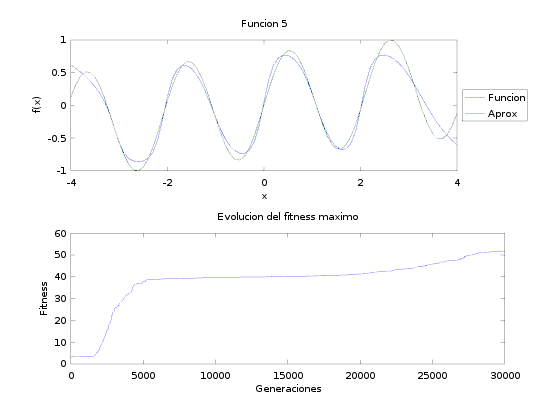
\includegraphics[width=0.85\textwidth]{img/56.png}
\caption{\label{fig:56} Prueba 2 de la tabla \ref{table:prueba2-met2}}
\end{figure}

\begin{figure}[h]
\centering
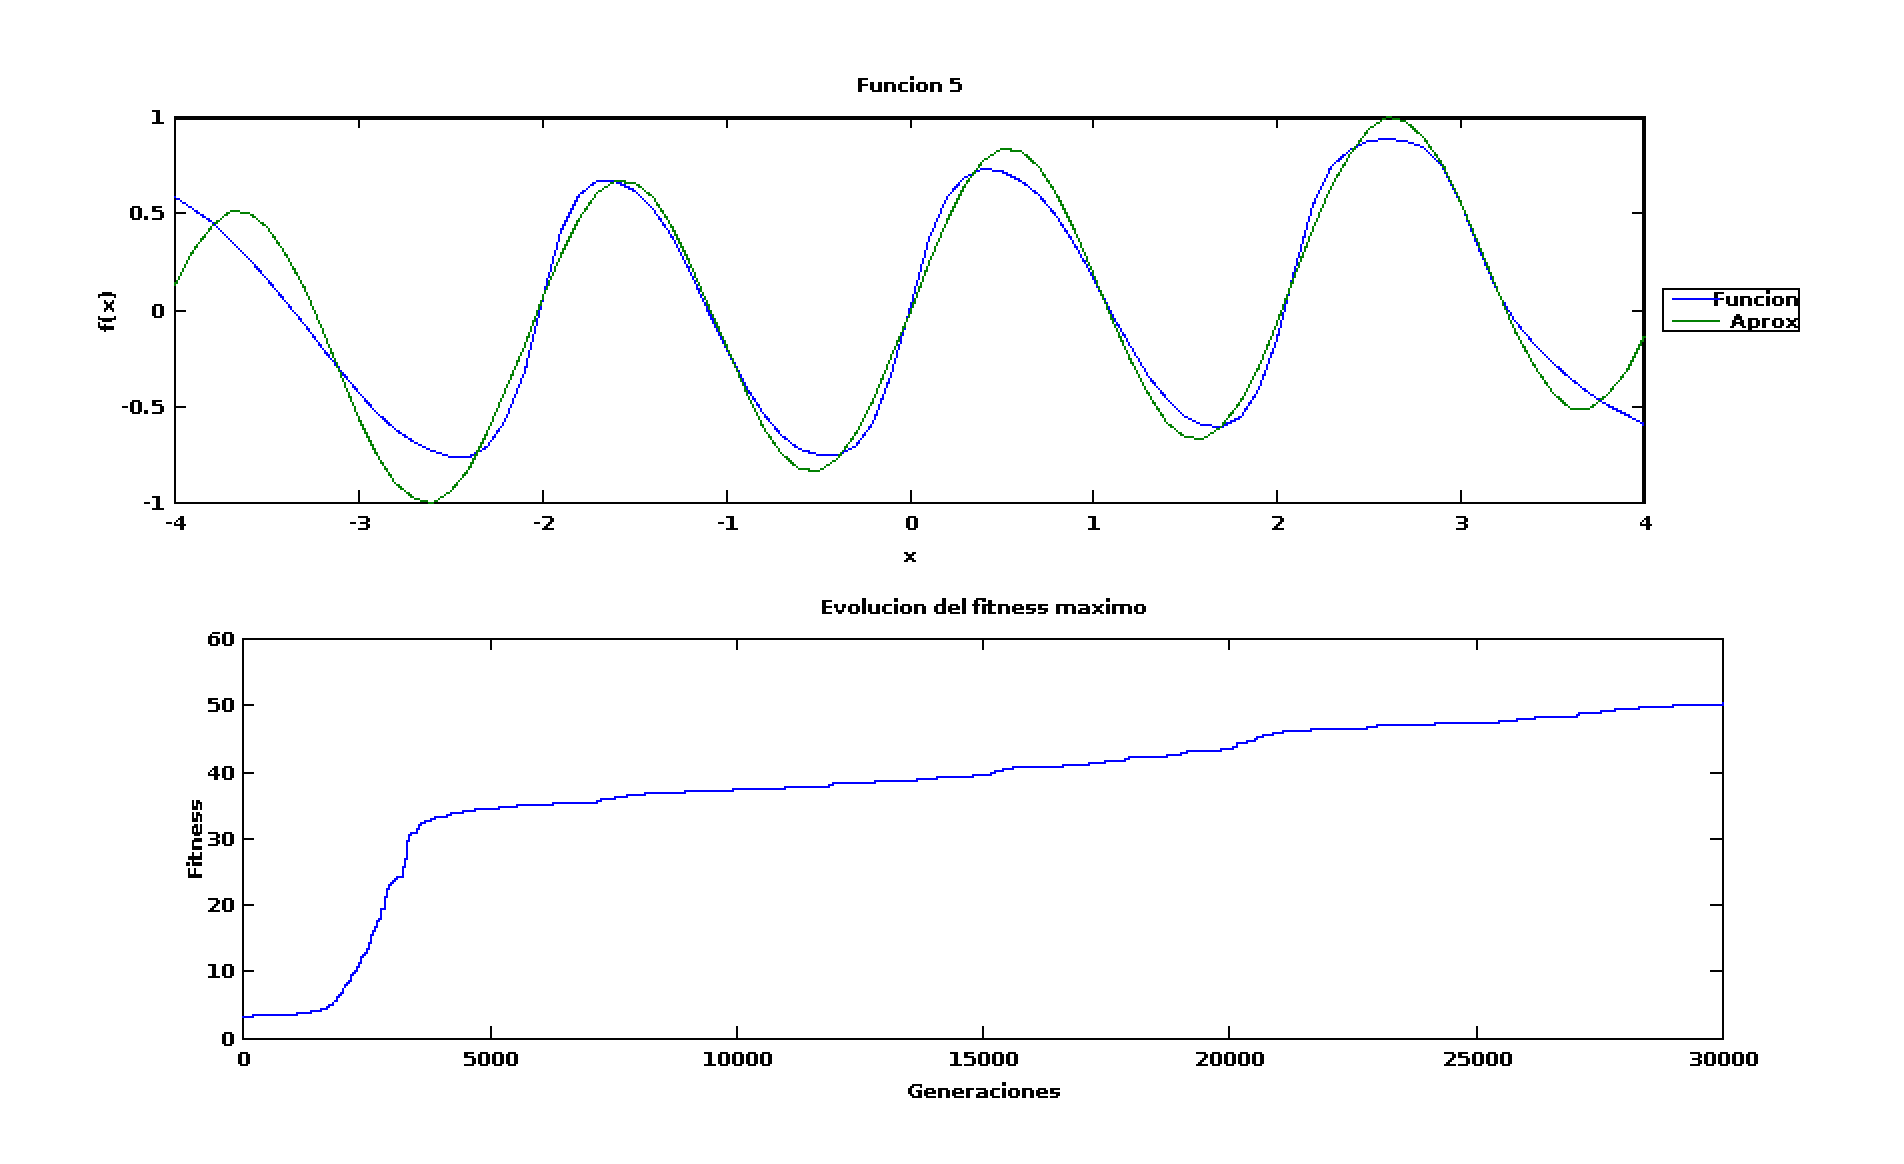
\includegraphics[width=0.85\textwidth]{img/9.png}
\caption{\label{fig:9} Prueba 3 de la tabla \ref{table:prueba2-met2}}
\end{figure}

\begin{figure}[h]
\centering
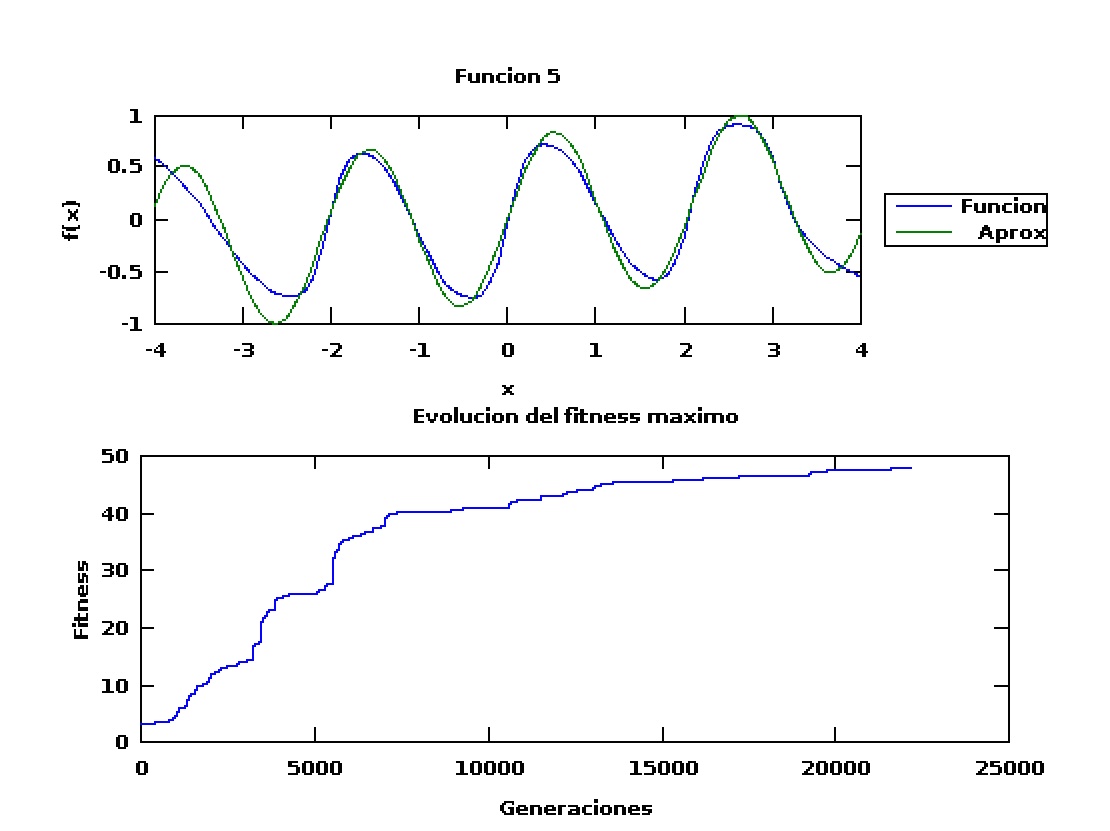
\includegraphics[width=0.85\textwidth]{img/5.png}
\caption{\label{fig:5} Prueba 4 de la tabla \ref{table:prueba2-met2}}
\end{figure}

\begin{figure}[h]
\centering
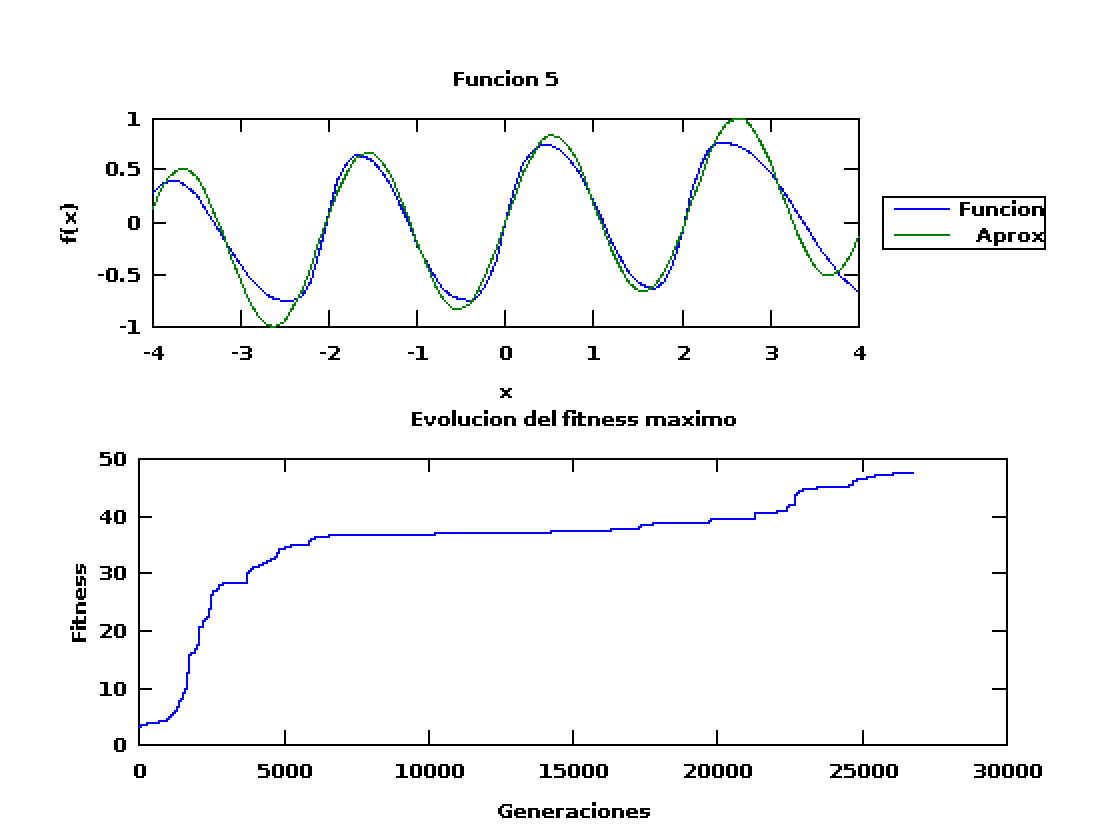
\includegraphics[width=0.85\textwidth]{img/59.png}
\caption{\label{fig:59} Prueba 5 de la tabla \ref{table:prueba2-met2}}
\end{figure}

\begin{figure}[h]
\centering
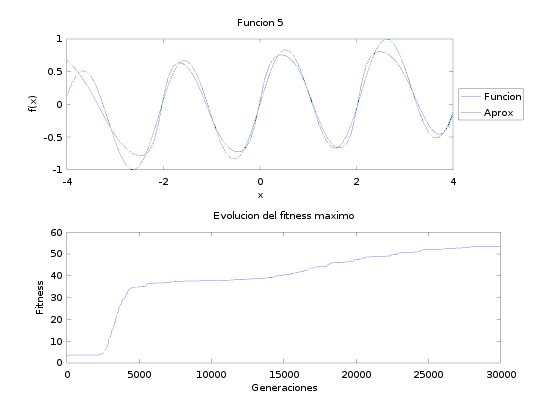
\includegraphics[width=0.85\textwidth]{img/39.png}
\caption{\label{fig:39} Prueba 1 de la tabla \ref{table:prueba2-met3}}
\end{figure}

\begin{figure}[h]
\centering
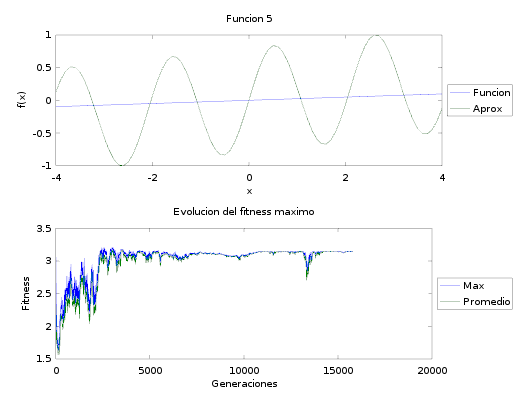
\includegraphics[width=0.85\textwidth]{img/best-met1.png}
\caption{\label{fig:best-met1} Método de reemplazo 1, selección$=$ \emph{Boltzman}, reemplazo$=$ \emph{Mixed con roulette} y $n=6$, cruza$=$ \emph{Two point cross}, probabilidad de mutación$=0.1$, mutación$=$ clásica, rango $=0.1$, generaciones $= 20000$.}
\end{figure}

\begin{figure}[h]
\centering
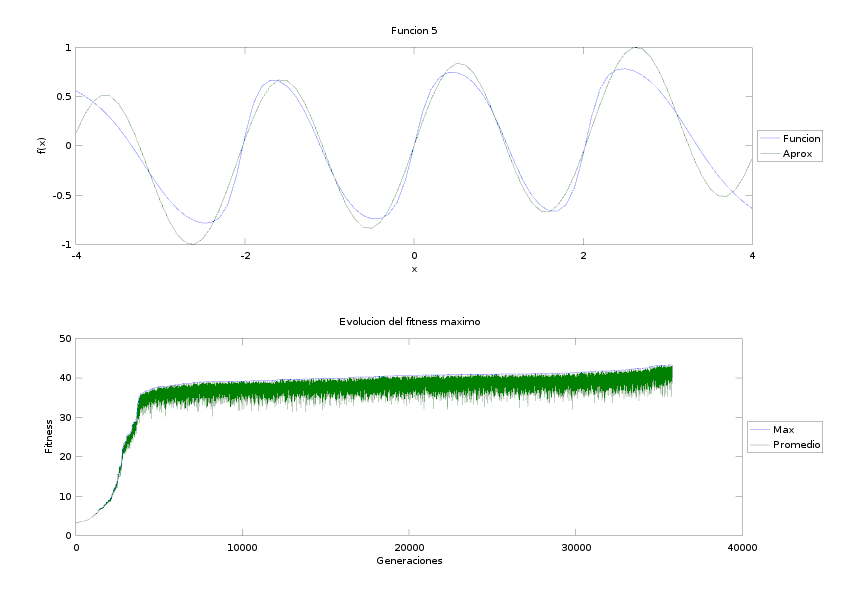
\includegraphics[width=0.85\textwidth]{img/best-met3.png}
\caption{\label{fig:best-met3} Método de reemplazo 3, selección$=$ \emph{Boltzman}, reemplazo$=$ \emph{Mixed con roulette} y $n=6$, cruza$=$ \emph{Two point cross}, probabilidad de mutación$=0.1$, mutación$=$ clásica, rango $=0.1$, generaciones $= 40000$.}
\end{figure}

\begin{figure}[h]
\centering
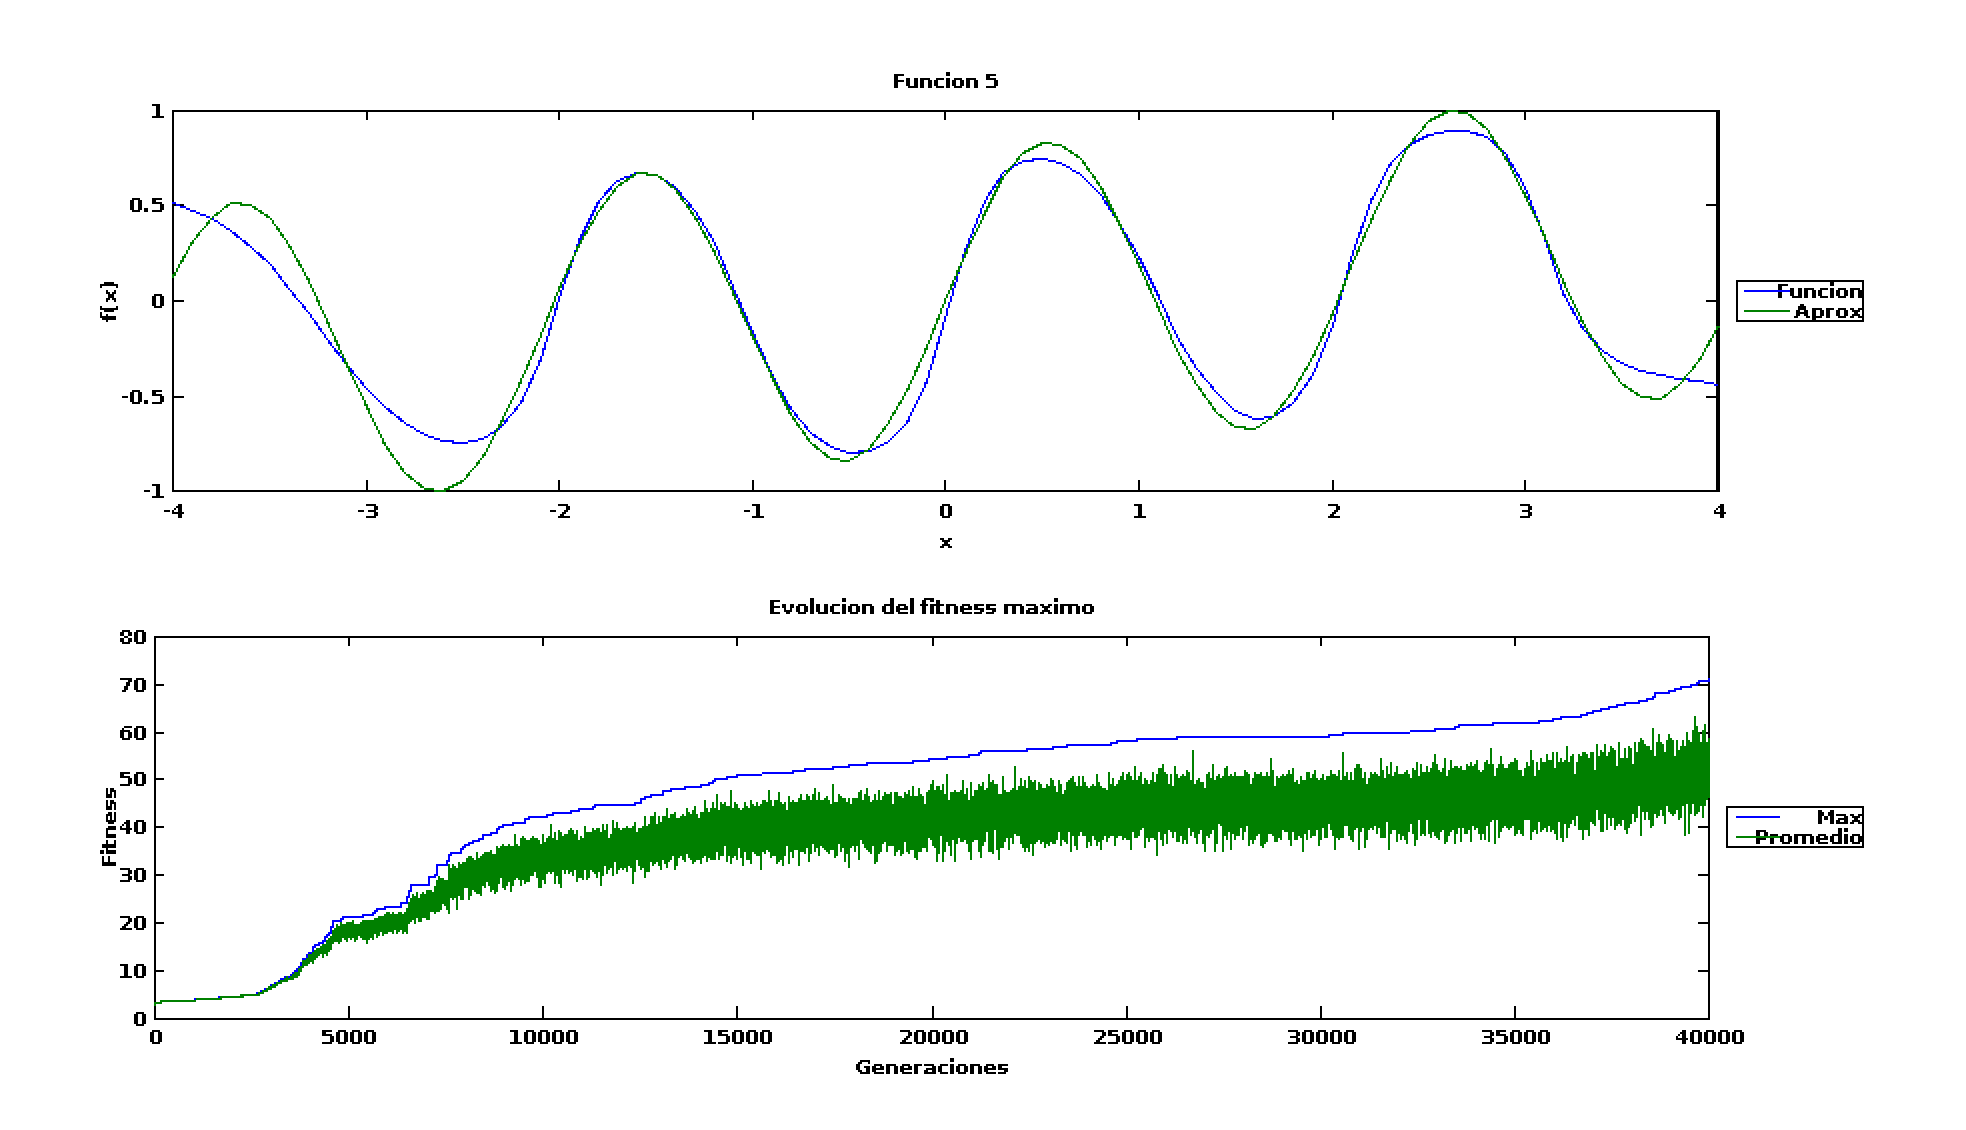
\includegraphics[width=0.85\textwidth]{img/mejor-config-40000-gen.png}
\caption{\label{fig:mejor-4000} Prueba 10 de la tabla \ref{table:pruebaF1} Método de reemplazo 2, selección$=$ \emph{Boltzman}, reemplazo$=$ \emph{Mixed con roulette} y $n=6$, cruza$=$ \emph{Two point cross}, probabilidad de mutación$=0.1$, mutación$=$ clásica, rango $=0.1$, generaciones $= 40000$.}
\end{figure}

\begin{figure}[h]
\centering
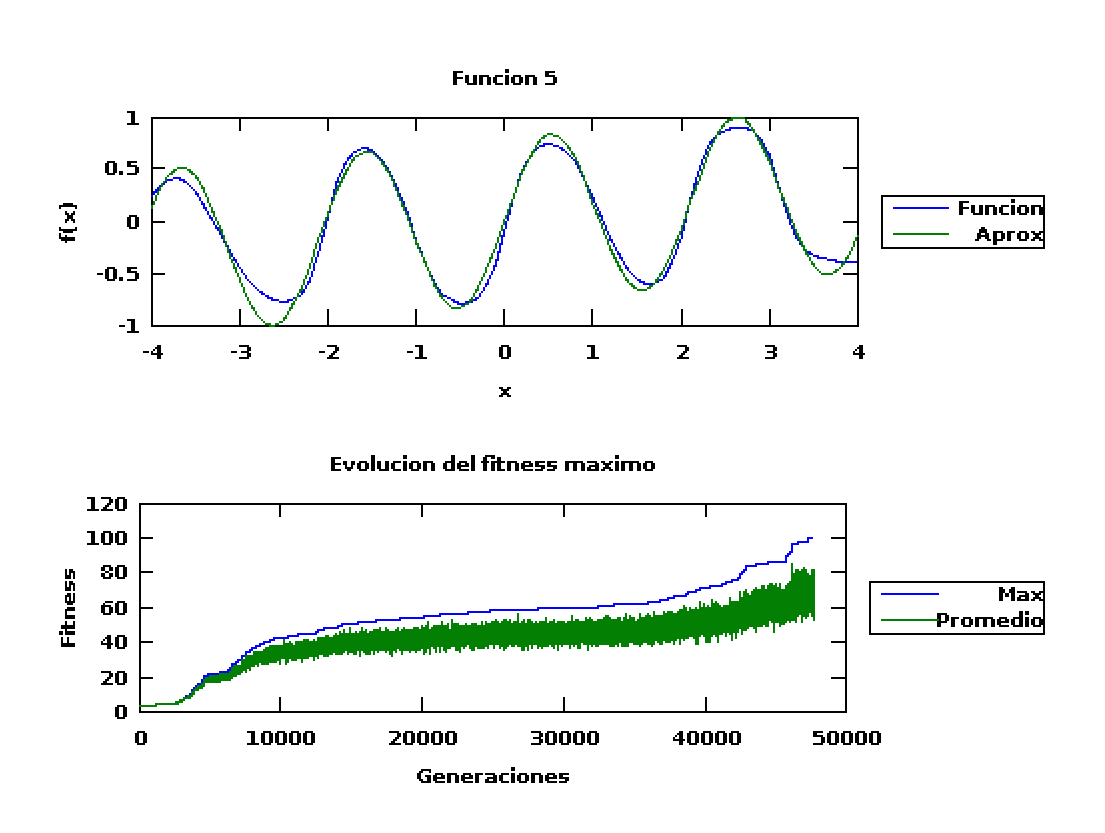
\includegraphics[width=0.85\textwidth]{img/mejor-config-corto-100.png}
\caption{\label{fig:mejor-corto-100} Prueba de la mejor configuración. Método de reemplazo 2, selección$=$ \emph{Boltzman}, reemplazo$=$ \emph{Mixed con roulette} y $n=6$, cruza$=$ \emph{Two point cross}, probabilidad de mutación$=0.1$, mutación$=$ clásica, rango $=0.1$, generaciones $= 60000$.}
\end{figure}


\begin{figure}[h]
\centering
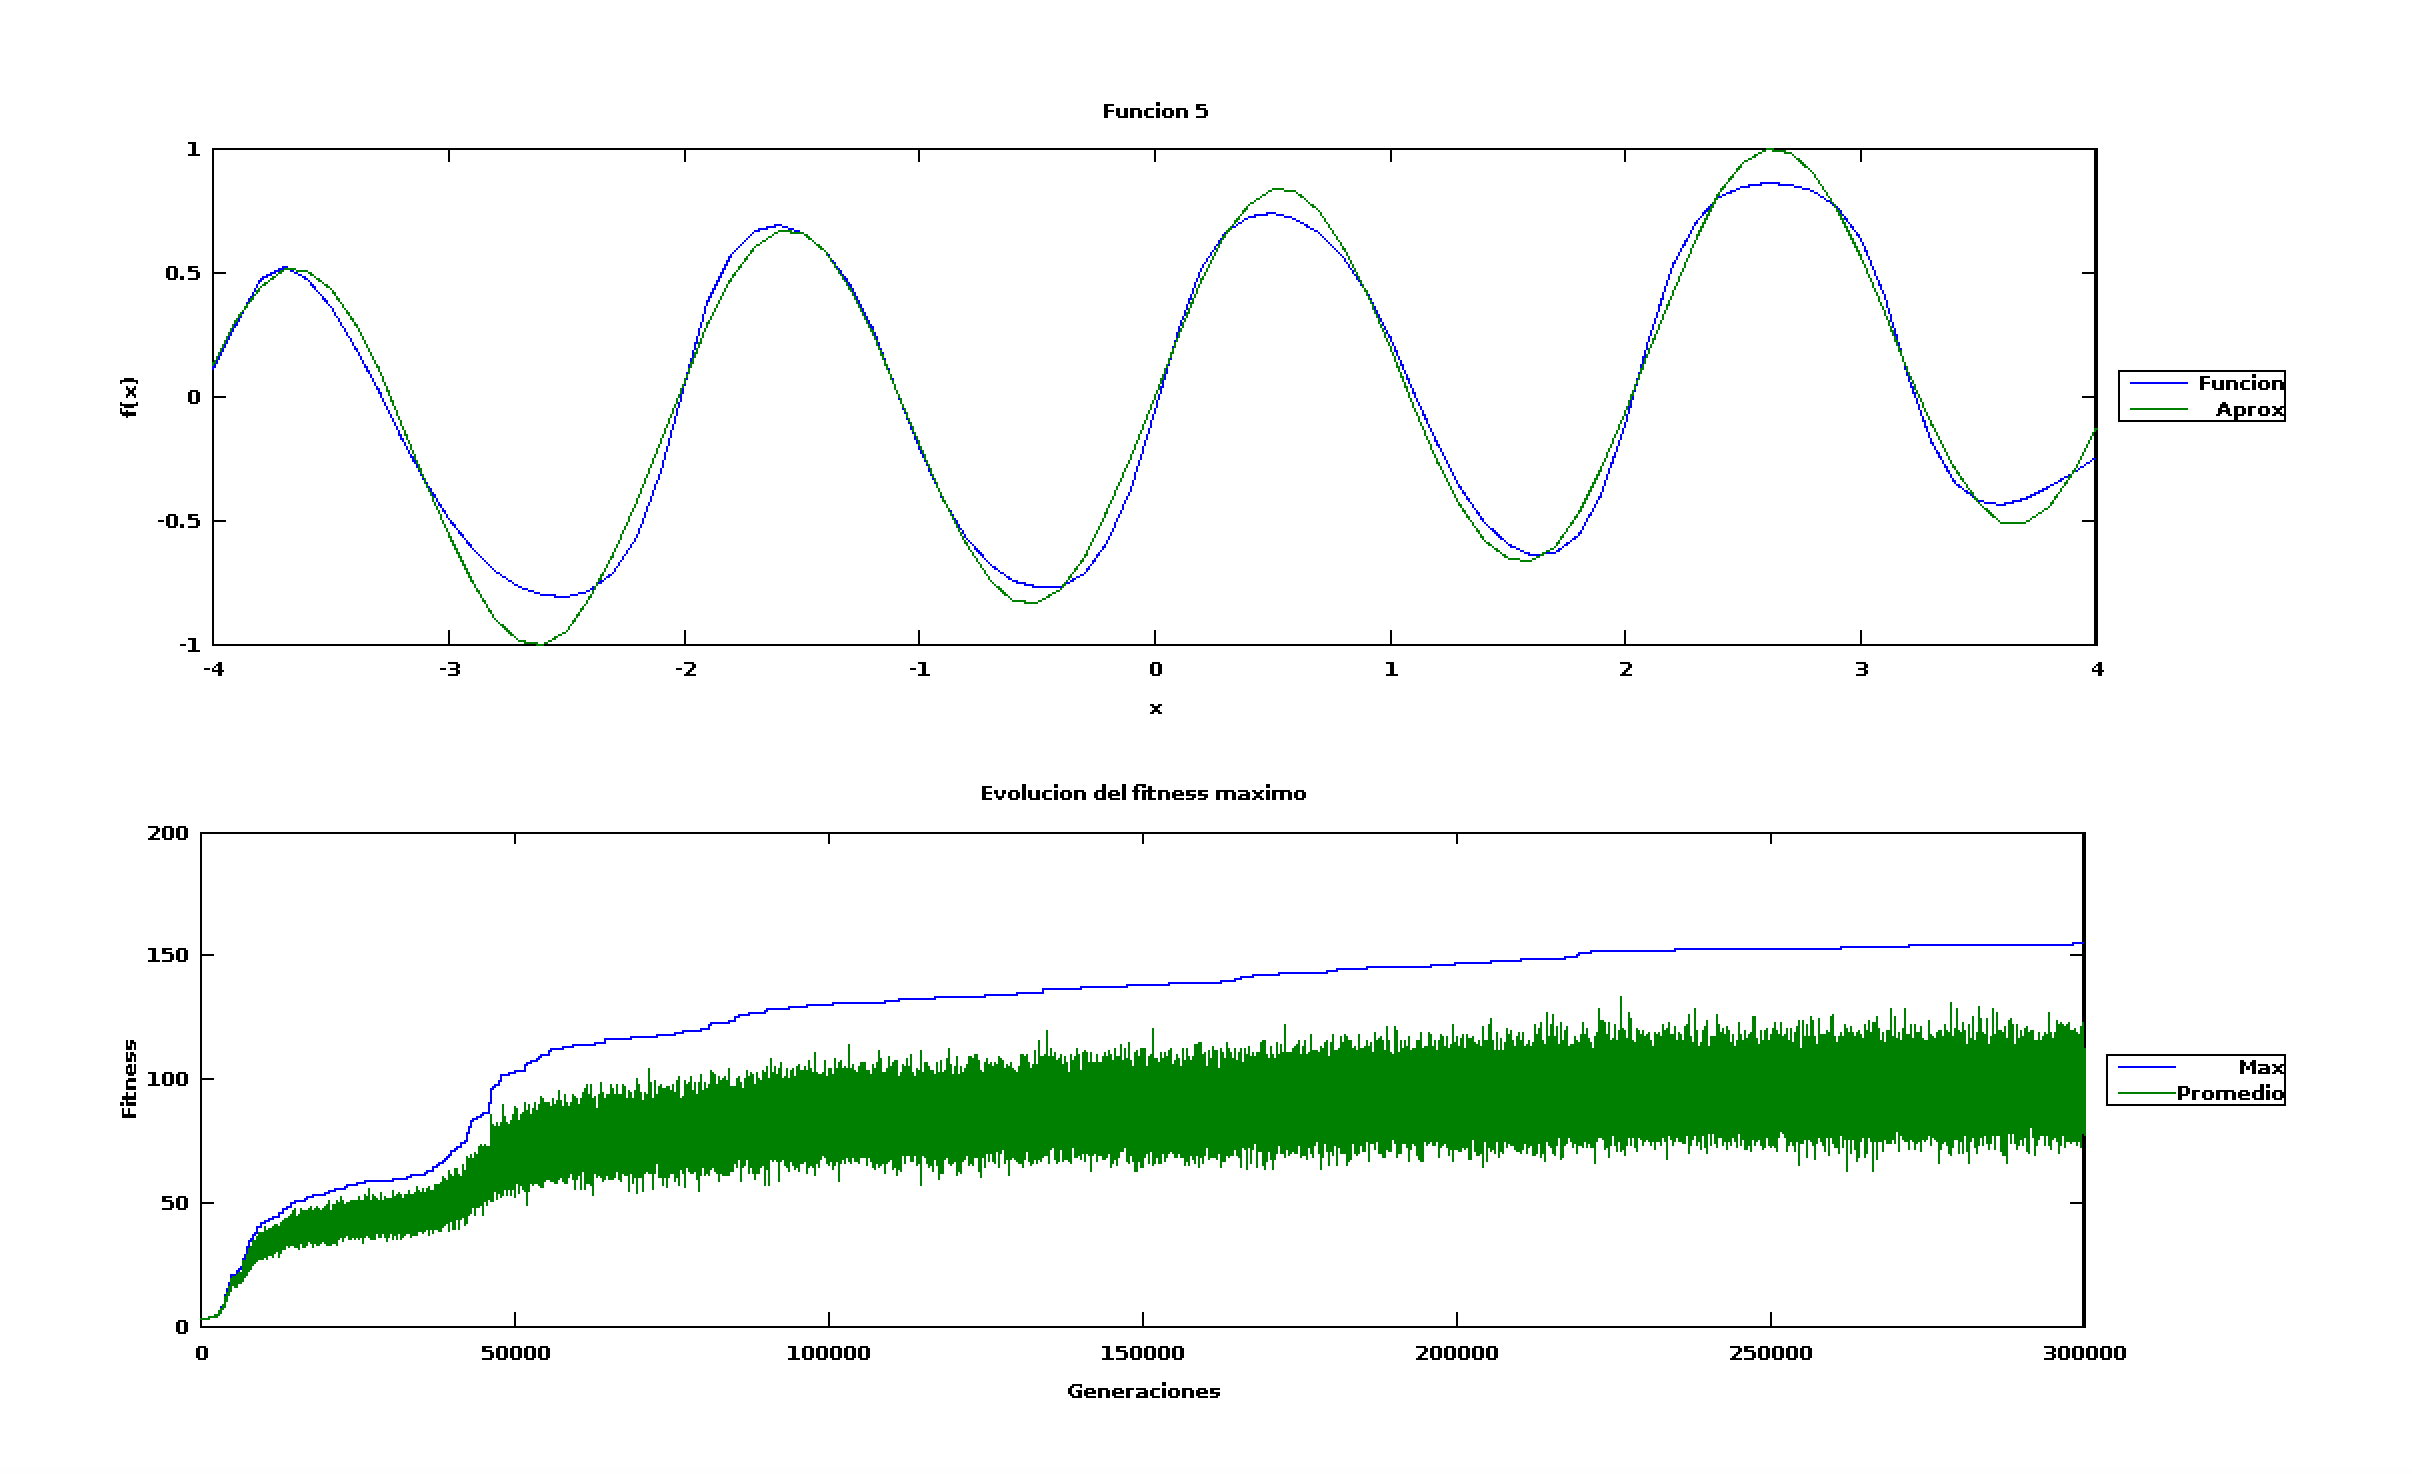
\includegraphics[width=0.85\textwidth]{img/mejor-config-300000-gen.png}
\caption{\label{fig:mejor-300000} Prueba de la mejor configuración en $300000$ generaciones. Selección$=$ \emph{Boltzman}, reemplazo$=$ \emph{Mixed con roulette} y $n=6$, cruza$=$ \emph{Two point cross}, probabilidad de mutación$=0.1$, mutación$=$ clásica, rango $=0.1$, generaciones $= 300000$. No se utilizaron otras condiciones de corte.}
\end{figure}


\end{document}